\section{...}

We will examine the so-called total domatic number of graphs.
Let $G = (V, E)$ be a graph without isolated vertices.

\begin{definition}
  $S \subseteq V$ is a total dominating set if every vertex has a neighbor in
  $S$. The total domatic number of $G$ is the maximum number of disjoint total
  dominating sets.
\end{definition}

Sometimes it's more convenient to look at total dominating sets as color classes.

\begin{definition}
  A coloring of the vertices is called a $k$-coupon coloring if every vertex
  has a neighbor from each color class. The coupon coloring number of $G$ is
  the maximum $k$ for which a $k$-coupon coloring exists. The coupon coloring
  number is denoted by $\chi_c(G)$.
\end{definition}

It turns out that determining the total domatic number (or equivalently the
coupon coloring number) of a graph is rather hard.

\begin{thm}
  It's NP-complete to decide whether the total domatic number of
  a graph is at least $2$.
\end{thm}

\begin{proof}
  ...
  (https://pdfs.semanticscholar.org/d44c/a18638eadeeb17b69f657cfa06c313646b8c.pdf
  or for bipartite:
  https://people.cs.clemson.edu/~goddard/papers/twoTotalDominationAugment.pdf)
\end{proof}

\section{Degree restrictions}

A natural question is whether graphs with an appropriately big minimum degree
always have a total domatic number of at least $2$.

\begin{thm}
  For every $d$ there exists a graph with minimum degree $d$ and without $2$
  disjoint total dominating sets.
\end{thm}
\begin{proof}
  ...
\end{proof}

...Other degree stuff (k-regular, maxdeg-mindeg small enough)...

\section{A conjecture of Goddard and Henning}

From now on we will focus on $2$-coupon colorings and planar graphs. A
conjecture of Goddard and Henning is the following.

\begin{conj}
  If $G$ is a simple triangulated planar graph of order at least $4$, then the
  total domatic number of $G$ is at least $2$.
\end{conj}

\begin{remark}
  The simplicity of the graph is necessary. Suppose the graph below has a
  $2$-coupon coloring. Then $A$ and $C$ must have different colors, because
  they are the only neighbors of $B$. Similarly, $C$ and $E$ must have different
  colors, as well as $E$ and $A$. That's a contradiction, since $A$, $C$ and
  $E$ form a triangular.
\end{remark}

\begin{figure}[h]
  \centering
  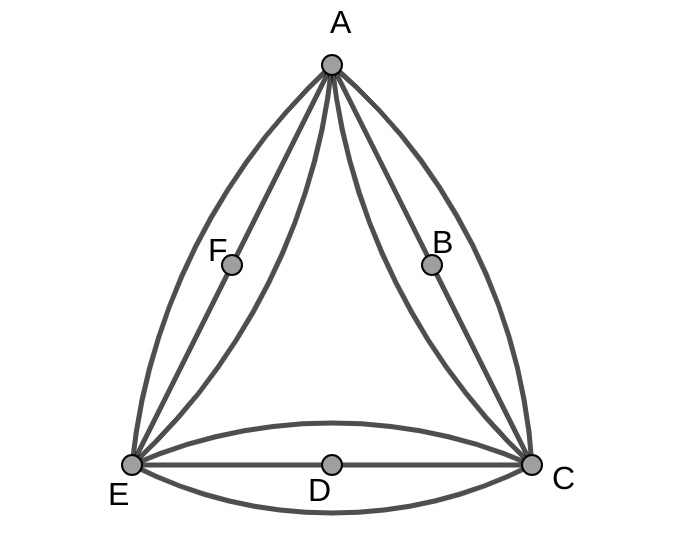
\includegraphics[width=70mm]{parallel}
\end{figure}

\begin{remark}
  Allowing triangulated disks (i.e. planar graphs with at most one face greater
  than $3$), the conjecture doesn't hold. For example, the graph below doesn't
  have a $2$-coupon coloring from similar reasons as the previous one. We will
  show later that this graph is a member of a bigger graph family without $2$
  disjoint dominating sets.
\end{remark}

\begin{figure}[h]
  \centering
  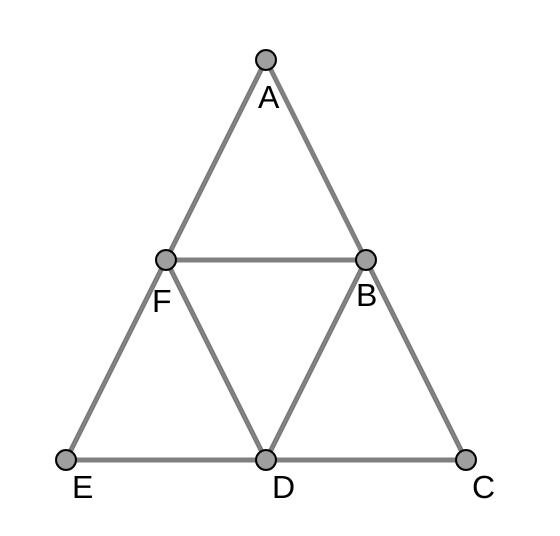
\includegraphics[width=70mm]{sungraph}
\end{figure}

\begin{thm}
  Let $G$ be a triangulated planar graph. If all the vertices of $G$ have an
  odd degree, then there exists a coupon coloring with $2$ colors.
\end{thm}
\begin{proof}
  ...
\end{proof}

\begin{thm}
  Outerplanar graphs ...
\end{thm}

\begin{thm}
  Every triangulated graph with a Hamiltonial circle admits 2 disjoint
  dominating sets.
\end{thm}

Hypergraph connection...
